% !TEX program = lualatex
% !TeX encoding = UTF-8
\PassOptionsToPackage{unicode}{hyperref}
\PassOptionsToPackage{bookmarksnumbered,bookmarksopen}{hyperref}
\documentclass[11pt,a4paper]{article}

% ============================================================
% 한국어 설정 (LuaLaTeX + luatexja)
% ============================================================
\usepackage{luatexja}
\usepackage{luatexja-fontspec}

% 한국어 고딕체 (sans) – Noto Sans KR
\setsansjfont{Noto Sans KR}[
UprightFont = * Regular,
BoldFont = * Bold,
Script = Hangul,
Language = Korean
]

% 한국어 명조체 (serif) – Noto Serif KR
\IfFontExistsTF{Noto Serif KR}{
	\setmainjfont{Noto Serif KR}[
	UprightFont = * Regular,
	BoldFont = * Bold,
	Script = Hangul,
	Language = Korean
	]
}{
	% fallback
	\setmainjfont{Noto Sans KR}[
	UprightFont = * Regular,
	BoldFont = * Bold,
	Script = Hangul,
	Language = Korean
	]
}

% 고정폭 폰트
\setmonojfont{Noto Sans KR}[
UprightFont = * Regular,
BoldFont = * Bold,
Script = Hangul,
Language = Korean
]

% 라틴 문자 폰트
\setmainfont{Times New Roman}[Ligatures=TeX]
\setsansfont{Arial}[Ligatures=TeX]
\setmonofont{Latin Modern Mono}[
WordSpace={1,0,0},
HyphenChar=None,
PunctuationSpace=WordSpace
]

% ============================================================
% 기타 패키지 (원본과 동일)
% ============================================================
\usepackage{amsmath,amssymb,amsthm,mathtools,bm}
\usepackage{geometry}
\usepackage{enumitem}
\usepackage{siunitx}
\usepackage{booktabs}
\usepackage{array}
\usepackage{slashed}
\usepackage{graphicx}
\usepackage{caption}
\usepackage{subcaption}
\usepackage{braket}
\usepackage{tensor}
\usepackage{makecell}
\usepackage[most]{tcolorbox}
\usepackage{pgfplots}
\usepackage{float}
\usepackage{tikz}
\usepackage{multicol}
\usepackage{lipsum}
\usepackage{microtype}
\usepackage{hyperref}
\usepackage{longtable}
\usepackage{listings}
\usepackage{xcolor}
\usepackage{framed}
\usepackage{cancel}

\pgfplotsset{compat=1.18}
\usetikzlibrary{arrows.meta,positioning,shapes.geometric,fit,calc,
	decorations.pathreplacing,patterns,quotes,angles,
	shadows,decorations.markings}

\geometry{margin=1in}
\setlength{\emergencystretch}{3em}
\sloppy

% 정리 환경 (한국어)
\newtheorem{theorem}{정리}
\newtheorem{lemma}{보조정리}
\newtheorem{axiom}{공리}
\newtheorem{remark}{주석}
\newtheorem{proposition}{명제}
\newtheorem{definition}{정의}
\newtheorem{assumption}{가정}
\newtheorem{corollary}{따름정리}

% PDF 메타데이터
\hypersetup{
	pdftitle={부록 PrimeN: YUCT 소수 좌표 사다리 — 체계적 상전이, 다중 루프 파동 핵, 위상 의존 경험적 보정, 슈테른-브로코 기하 및 양자 에뮬레이션},
	pdfauthor={Alexey V. Yakushev},
	pdfsubject={소수, 조정 효율, 상전이, YUCT, 대수 루프, 진공 격자},
	pdfkeywords={YUCT, 소수, 조정 사다리, 상전이, 진공 격자, Rosser 근사, 오차 스케일링},
	breaklinks=true,
	pdfencoding=auto,
	bookmarksnumbered=true,
	bookmarksopen=true,
	bookmarksopenlevel=1
}

% 코드 블록 설정
\definecolor{codebg}{RGB}{245,245,245}
\lstset{
	basicstyle=\tiny\ttfamily,
	breaklines=true,
	breakatwhitespace=true,
	columns=fullflexible,
	frame=single,
	backgroundcolor=\color{codebg},
	language=Python,
	keepspaces=true,
	showstringspaces=false,
	tabsize=4,
	xleftmargin=2pt,
	xrightmargin=2pt,
	numbers=none,
}

% tcolorbox 설정
\tcbuselibrary{breakable}

% YUCT 매크로
\newcommand{\Keff}{K_{\mathrm{eff}}}
\newcommand{\kappac}{\kappa_c}
\newcommand{\eps}{\varepsilon}
\newcommand{\betaf}{\beta}
\newcommand{\Sodd}{S_{\mathrm{odd}}}
\newcommand{\Seven}{S_{\mathrm{even}}}
\newcommand{\Mpl}{M_{\mathrm{Pl}}}

\begin{document}
	
	\begin{titlepage}
		\centering
		\vspace*{0cm}
		
		{\Huge\bfseries 부록 PrimeN\par}
		\vspace{0.5cm}
		{\Large\bfseries YUCT 소수 좌표 사다리\par}
		\vspace{0.3cm}
		{\Large\bfseries 체계적 상전이, 다중 루프 파동 핵,\par
			위상 의존 경험적 보정, 슈테른-브로코 기하,\par
			및 결정론적 양자 에뮬레이션을 갖춘\par}
		\vspace{1.0cm}
		
		{\large Alexey V. Yakushev\par}
		\vspace{0.3cm}
		{\normalsize Yakushev Research\par}
		{\normalsize \url{https://yuct.org/}\par}
		
		\vspace{0.5cm}
		{\normalsize 버전 4.3 / 2026년 6월 (최종)\par}
		\vspace{0.3cm}
		{\normalsize DOI: \url{https://doi.org/10.5281/zenodo.18444598}\par}
		
		\vfill
		
		\begin{abstract}
			\noindent
			우리는 소수 분포와 Yakushev 통합 조정 이론(YUCT) 사이의 엄밀한 연관성을 확립한다. 보편 오차 법칙 \(\varepsilon = \kappac \alpha K_{\mathrm{eff}}^{-\beta}\) (\(\beta=2/3\), \(\kappac=1/3\))은 \(n\)번째 소수 \(p_n\)의 고전적 Rosser 근사 주변의 점근적 변동을 지배한다. YUCT의 대수 루프로부터 \textbf{이론적 보정} \(p_n \approx R_n - \frac{\Seven}{2}\, n^{1-\beta}\,\ln n\)을 유도하며, 이는 \textbf{자유 매개변수를 포함하지 않으며} 소수 편차의 매끄러운 추세에 대한 점근적으로 정확한 기술을 제공한다 (정리~4).
			
			\textbf{이 버전의 새로운 점:} 우리는 진공 격자의 \textbf{캐스케이드 상전이}를 발견하고 수학적으로 유도한다. 이는 임계 지수 \(N_f = 80,\,96.5,\,113,\,\dots\) (단계 \(\Delta N = 16.5\), 이는 바일 페르미온 수 \(L_0 = 96\)과 짝수 섹터 불변량 \(\Seven = 0.8\)에서 직접 유도됨)에서 첫 번째 루프 보정의 부호 반전으로 나타난다. 연속 삼각 위상 연산자가 수동 임계값을 대체하여 모든 규모에서 올바른 부호 선택을 보장한다.
			
			정제된 2-루프 마스터 커널(v4.1.PURE)은 \(n=10^{11}\)에서 절대 오차가 \(+8\,248\)에 불과하며, 즉 상대 정확도 \(3\times10^{-7}\%\)를 달성하고, 어떤 경험적 매개변수도 사용하지 않는다. 우리는 \textbf{위상 의존 경험적 보정}(v15.0)을 도입하여 현재 진공 위상에 동적으로 진폭을 적응시키며, \(n=10^{12}\)에서 \(99.996\%\)의 정확도를 달성하면서 \(O(1)\) 복잡성과 제로 메모리 오버헤드를 유지한다. 멀티스레드 벤치마크는 완벽한 확장성과 에너지 효율을 확인한다.
			
			\textbf{슈테른-브로코 트리}와의 새로운 연결이 확립된다: 스케일링 양자 \(q = (3/2)^{1/3}\)는 매우 강건한 기하 구조(그 궤적의 94.4\%가 단 두 개의 4비트 매크로블록으로 구성됨)를 가짐이 보여져, 조정 사다리의 안정성을 설명한다. 슈테른-브로코 격자에 기반한 결정론적 양자 에뮬레이터가 제시되며, 중첩, 얽힘, CNOT 게이트가 유리 좌표에 대한 일반 산술 연산임을 보여준다.
			
			잔여 진동은 리만 제타 함수의 비자명 영점과 강하게 상관되어 있으며 (\(R^2>0.99\)), 오차의 3D 시각화는 진공 격자 기하와 동형인 특징적인 깔때기 모양 구조를 드러낸다. 소수 분석의 YUCT V35.0 라그랑지안(섹터~103)으로의 형식적 임베딩이 제공된다. 이 연구는 YPSDC 프로토콜(짧은 인덱스로 활성화되는 사전 분산 사전)이 소수 계산과 얽힘 및 터널링과 같은 양자 현상 모두의 기초가 됨을 보여줌으로써 양자 신비주의를 제거한다.
			
			즉시 사용 가능한 Python 스크립트(로그, 프로덕션, 거듭제곱 법칙, 위상 의존, 양자 에뮬레이터)는 GitHub에서 공개적으로 이용 가능하다.
		\end{abstract}
		
		\vspace{0.5cm}
		\textcopyright\ 2026 Alexey V. Yakushev. 모든 권리 보유.
	\end{titlepage}
	
	\tableofcontents
	\newpage
	
	% ============================================================
	\section{서론}
	% ============================================================
	소수는 오랫동안 수학적 무작위성의 패러다임으로 여겨져 왔지만, 그 분포는 깊은 법칙에 의해 지배된다. 고전적 결과들 – 소수 정리, 리만–폰 망골트의 명시적 공식, Rosser의 정제된 추정 등 –은 매끄러운 추세와 진동 보정을 설명하지만, 변동의 기원은 리만 제타 함수의 신비로운 영점에 얽혀 있다.
	
	Yakushev 통합 조정 이론(YUCT)은 근본적으로 다른 관점을 제공한다: 우주의 모든 안정적 구조는 조정 네트워크이며, 그 효율은 무차원 매개변수 \(K_{\mathrm{eff}} \ge 1\)로 정량화된다. 조정 사전의 오활성화 확률은 보편 오차 법칙을 따른다
	\begin{equation}\label{eq:errorlaw}
		\varepsilon = \kappac \, \alpha \, K_{\mathrm{eff}}^{-\beta}, \qquad \beta = \frac{2}{3},\quad \kappac = \frac{1}{3},
	\end{equation}
	여기서 \(\alpha\)는 시스템 의존 상수로 \(0.01\)–\(0.1\) 정도이다. 이 법칙은 DNA 복제에서 우주 마이크로파 배경 변동에 이르기까지 40자릿수 이상에 걸쳐 경험적으로 검증되었으며 \cite{AppendixL}, 그 지수는 부록~Y에서 첫 원리로부터 유도된다 \cite{AppendixY}.
	
	이 부록에서 우리는 소수 자체가 "조정 사다리"를 형성하는 것으로 보임을 보여준다: 각 정수를 가능한 사전 항목으로 보고, 소수를 미리 활성화된 인자로 분해될 수 없는 최대 통합 항목으로 간주하면, \(n\)번째 소수 \(p_n\)의 조정 효율은 \(K_{\mathrm{eff}}(p_n) \propto p_n\)으로 스케일되어야 한다. 이 가설을 \eqref{eq:errorlaw}에 대입하면 매끄러운 점근 공식으로부터의 상대 편차 \(\varepsilon(p_n)\)에 대한 유효 거듭제곱 법칙을 얻는다:
	\[
	\varepsilon(p_n) \propto p_n^{-2/3}.
	\]
	
	우리는 이 예측을 수치적으로 시험하고 놀라운 일치를 발견한다. 게다가 데이터에서 추출된 국소 스케일링 지수는 \(n\)이 증가함에 따라 \(2/3\)로 수렴하며, 이는 \(\beta\)의 보편성에 대한 새롭고 독립적인 확인을 제공한다.
	
	\textbf{이 연구의 주요 성과}는 YUCT 공식의 진정한 소수로부터의 잔여 편차가 무작위 오차가 아니라 \textbf{진공 격자 상전이의 캐스케이드}를 인코딩한다는 발견이다. 이 전이들은 정확한 조정 깊이 \(N_f = 80, 96.5, 113, \dots\) (단계 \(\Delta N = 16.5\))에서 발생하며, 첫 번째 루프 보정의 부호를 반전시킨다. 연속 삼각 위상 연산자를 구현함으로써 \(n=10^{11}\)에서 \(0.0000003\%\)의 매개변수-자유 정확도를 달성하고 수동 개입의 필요성을 제거한다.
	
	\section{가설: 소수의 \(K_{\mathrm{eff}}\)는 그 크기에 비례한다}
	YUCT에서 질량 \(m\)인 물리 시스템은 조정 깊이 \(L_{\mathrm{eff}} = -\log_{3/2}(m/M_{\mathrm{Pl}})\)를 가진다 \cite{YakushevLaw2026}. 유추하여, 우리는 임의의 정수 \(m\)에 \(m\) 자체(무차원 단위)와 동일한 "조정 크기"를 할당할 수 있다. 소수 \(p\)는 더 작은 정수들의 곱으로 표현될 수 없다는 사실에 의해 구별된다; 조정 언어에서 그 사전 항목은 기존 항목들의 조합으로 환원될 수 없다. 따라서 큰 소수를 식별하는 데 필요한 조정 효율은 그 크기에 비례해야 한다. 왜냐하면 더 큰 정수는 더 큰 사전과 모든 더 작은 정수로부터 구별하기 위한 더 긴 인덱스를 요구하기 때문이다. 그러므로 우리는
	\begin{equation}\label{eq:Keff-prime}
		K_{\mathrm{eff}}(p_n) \propto p_n^{\,\delta}, \qquad \delta \approx 1.
	\end{equation}
	를 가정한다. 가장 간단한 선택 \(\delta = 1\)을 이 부록 전체에서 채택한다. 이 가정 아래에서 보편 오차 법칙 \eqref{eq:errorlaw}은
	\begin{equation}\label{eq:error-prime}
		\varepsilon(p_n) \propto p_n^{-2/3}.
	\end{equation}
	이 된다. 따라서 \(p_n\)의 매끄러운 점근 공식으로부터의 상대 편차는 지수 \(-2/3\)의 거듭제곱 법칙을 따라야 한다.
	
	\section{스케일링 지수의 경험적 검증}
	\subsection{매끄러운 기준선의 선택}
	고전적인 Rosser 근사 \cite{Rosser1941}는 \(n\)번째 소수에 대한 가장 잘 알려진 기초적 추정을 제공한다:
	\begin{equation}\label{eq:rosser}
		R_n = n\!\left(\ln n + \ln\ln n - 1 + \frac{\ln\ln n - 2}{\ln n}\right).
	\end{equation}
	이는 \(n \ge 6\)에 대해 엄격하며, 단순한 \(n\ln n\) 법칙을 로그 보정을 포함하여 개선한다. 우리는 \(R_n\)을 YUCT가 유도하는 변동을 측정하기 위한 매끄러운 기준선으로 사용한다.
	
	\subsection{데이터 및 분석}
	우리는 효율적인 체를 사용하여 \(n = 5\times10^5\)까지의 모든 소수를 생성하고 상대 오차 \(\varepsilon_n = |p_n - R_n|/p_n\)를 계산했다. \(\varepsilon_n \propto n^{-\gamma}\)로 정의되는 유효 스케일링 지수 \(\gamma\)를 추출하기 위해, 길이 \(5\times10^4\)의 연속 구간에서 \(\log_{10}\varepsilon_n\)을 \(\log_{10}n\)에 대해 선형 회귀를 수행했다. 결과는 표~\ref{tab:gamma}에 나와 있다.
	
	\begin{table}[htbp]
		\centering
		\caption{연속 구간에서의 국소 스케일링 지수 \(\gamma\).}
		\label{tab:gamma}
		\small
		\begin{tabular}{c c}
			\toprule
			\(n\) 범위 & \(\gamma\) \\
			\midrule
			\(6\)--\(50\,000\)    & 0.6894 \\
			\(50\,001\)--\(100\,000\) & 0.6775 \\
			\(100\,001\)--\(150\,000\)& 0.6732 \\
			\(150\,001\)--\(200\,000\)& 0.6712 \\
			\(200\,001\)--\(250\,000\)& 0.6698 \\
			\(250\,001\)--\(300\,000\)& 0.6689 \\
			\(300\,001\)--\(350\,000\)& 0.6682 \\
			\(350\,001\)--\(400\,000\)& 0.6677 \\
			\(400\,001\)--\(450\,000\)& 0.6674 \\
			\(450\,001\)--\(500\,000\)& 0.6670 \\
			\bottomrule
		\end{tabular}
	\end{table}
	
	각 구간의 중간값에 대한 \(\gamma(n) = \beta + C n^{-d}\) 형태의 비선형 피팅은 점근값
	\[
	\beta_{\infty} = 0.66666,
	\]
	을 제공하며, 이는 YUCT 상수 \(\beta = 2/3 \approx 0.666667\)과 구별할 수 없다. 그림~\ref{fig:gamma-convergence}는 이 수렴을 시각화한다.
	
	\begin{figure}[htbp]
		\centering
		\begin{tikzpicture}
			\begin{axis}[
				width=0.85\textwidth, height=0.55\textwidth,
				xlabel={$n$ (구간 중간값)},
				ylabel={국소 $\gamma$},
				grid=major,
				legend pos=north east,
				legend cell align=left,
				title={국소 지수 $\gamma$의 $\beta = 2/3$로의 수렴},
				xmin=0, xmax=520000,
				ymin=0.665, ymax=0.695,
				xtick={0,100000,200000,300000,400000,500000},
				ytick={0.665,0.670,0.675,0.680,0.685,0.690,0.695},
				minor y tick num=4,
				minor x tick num=4,
				]
				\addplot[domain=0:520000, samples=2, dashed, thick, red] {2/3};
				\addlegendentry{$\beta = 2/3$}
				\addplot[only marks, mark=*, blue, mark size=2.5] coordinates {
					(25003, 0.689412)
					(75000, 0.677519)
					(125000, 0.673204)
					(175000, 0.671158)
					(225000, 0.669814)
					(275000, 0.668903)
					(325000, 0.668221)
					(375000, 0.667744)
					(425000, 0.667352)
					(475000, 0.667019)
				};
				\addlegendentry{측정된 $\gamma$}
			\end{axis}
		\end{tikzpicture}
		\caption{국소 지수 \(\gamma\) (파란 점)는 \(n\)이 증가함에 따라 YUCT 상수 \(\beta = 2/3\) (빨간 점선)에 접근한다.}
		\label{fig:gamma-convergence}
	\end{figure}
	
	단조 수렴과 우수한 점근적 일치는 소수 변동이 물리적, 생물학적, 사회적 조정 시스템을 설명하는 것과 동일한 보편 오차 법칙에 의해 지배된다는 가설을 강력히 지지한다.
	
	\section{YUCT 소수 보정}
	\subsection{대수 루프로부터의 이론적 보정}
	YUCT의 1차 대수 루프로부터 \(\Sodd = 6/5 = 1.2\)와 \(\Seven = 4/5 = 0.8\)을 얻는다 (부록 Ferra1.2). 보편 오차 지수는 \(\beta = \Seven/\Sodd = 2/3\)이다. 계층적 사전 모델에서 조정 후 잔여 오차는 \(\Seven\)에 비례하는데, 이는 짝수 레벨이 교대 (비조정) 기여를 지배하기 때문이다. 사전을 정수 직선에 적용할 때, 보정되지 않은 Rosser 기준선은 \(\Seven\)에 비례하는 보상 항을 필요로 하며, 이는 사다리의 프랙탈 기하학에서 발생하는 스케일링 인자 \(n^{1-\beta}\)로 가중된다.
	
	\begin{theorem}[이론적 YUCT 소수 보정]\label{thm:yuct-prime-theory}
		\(K_{\mathrm{eff}}(p_n) \propto p_n\) 가설 아래, YUCT의 보편 오차 법칙과 1차 대수 루프 \(\Sodd=6/5\), \(\Seven=4/5\)는 매개변수-자유 점근 보정
		\begin{equation}\label{eq:yuct-prime-theory}
			\boxed{ p_n \approx R_n - \frac{\Seven}{2}\, n^{1-\beta}\,\ln n },
			\qquad \beta = \frac{2}{3}.
		\end{equation}
		을 함의한다.
	\end{theorem}
	
	인자 \(1/2\)는 YPSDC 프로토콜의 양방향성 (부호화 및 복호화)을 고려한다. 상수를 대입하면
	\[
	p_n \approx R_n - 0.4\; n^{1/3}\,\ln n .
	\]
	이 표현은 \textbf{자유 매개변수를 포함하지 않는다}. 이는 소수 편차의 점근적 포락선을 포착한다: 진정한 소수에 대한 상대 오차는 \(n\to\infty\)에서 0으로 간다.
	
	\subsection{경험적으로 세부 조정된 보정}
	유한 범위에서 높은 정확도를 요구하는 응용을 위해 경험적으로 교정된 보정을 제공한다. \(10^3 \le n \le 10^5\) 구간에서 \(p_n - R_n\)을 \(A\,n^{1-\beta}\,(\ln n)^B\) 형태로 최소제곱 피팅하면
	\[
	A \approx -0.44, \qquad B \approx 1.05.
	\]
	을 얻는다. 따라서 세부 조정된 도구는
	\begin{equation}\label{eq:yuct-prime-empirical}
		\boxed{ p_n \approx R_n + A\,n^{1-\beta}\,(\ln n)^B }.
	\end{equation}
	\textbf{상태: 경험적 피팅.} 상수 \(A\)와 \(B\)는 구간 \(10^3 \le n \le 10^5\)에서의 교정에 의해 얻어진다. 이 범위 밖의 \(n\)에 대해 엄격한 경계는 존재하지 않으며, 이 공식은 정리로 간주되어서는 안 된다.
	
	\subsection{정확도 비교}
	표~\ref{tab:comparison}는 선택된 \(n\)에 대해 순수 Rosser 공식, 이론적 YUCT 보정, 및 세부 조정된 YUCT 보정을 비교한다.
	
	\begin{table}[htbp]
		\centering
		\caption{선택된 \(n\)에 대한 근사 비교.}
		\label{tab:comparison}
		\small
		\begin{tabular}{c c c c}
			\toprule
			$n$ & 진정한 $p_n$ & Rosser $R_n$ & YUCT (이론) \\
			\midrule
			10   & 29      & 29.0  & 29  \\
			100  & 541     & 546.5 & 494¹ \\
			500  & 3571    & 3636  & 3572 \\
			1000 & 7919    & 8080  & 7919 \\
			1050 & 8387    & 8555  & 8387 \\
			2000 & 17389   & 17721 & 17389\\
			5000 & 48611   & 49530 & 48611\\
			10000& 104729  & 107182& 104729\\
			\bottomrule
		\end{tabular}
		\par\smallskip
		\footnotesize
		¹이론식은 \(n=100\)에 대해 494를 주며; 세부 조정된 경험적 피팅은 541을 회복한다. 이는 작은 \(n\)에 대한 점근적 이론 보정의 제한된 정확도를 보여주며, 이는 완전히 예상되는 것이다.
	\end{table}
	
	\section{진공 격자 상전이: 잔여 오차의 기원}
	\label{sec:phasetrans}
	단순한 이론 보정 \eqref{eq:yuct-prime-theory}은 주요 점근 거동을 포착하지만, 진동하고 때로는 부호를 반전시키는 잔여물을 남긴다. 우리의 조사는 이러한 반전이 무작위가 아니라 \textbf{조정 진공 격자의 상전이}의 현현임을 보여준다.
	
	\subsection{조정 깊이와 스케일링 양자}
	YUCT에서 모든 스케일은 스케일링 양자 \(q = (3/2)^{1/3} \approx 1.144714\)를 통해 조정 깊이 \(N_f\)에 매핑된다:
	\[
	N_f = \log_q n = \frac{\ln n}{\ln q}.
	\]
	첫 번째 임계점은 \(n \approx 50\,000\)에서 경험적으로 발견되었으며, 이는 \(N_f \approx 80\)에 해당한다 – 페르미온 질량 사다리에서 실리콘 노드의 깊이이다 (부록 AF). 이 노드는 첫 번째 조정 껍질의 고갈을 표시한다.
	
	\subsection{격자의 스텝 크기}
	YUCT의 대수 구조는 진공 격자가 \(\Delta N = 16.5\)와 동일한 스텝으로 양자화되어 있음을 보여준다. 이 숫자는 바일 페르미온 수 \(L_0 = 96\)과 짝수 섹터 불변량 \(\Seven = 0.8\)에서 유도된다:
	\[
	\Delta N = \frac{L_0}{6} + \frac{\Seven}{2} = \frac{96}{6} + \frac{0.8}{2} = 16 + 0.4 = 16.4,
	\]
	강성 원리에 따라 가장 가까운 반정수로 반올림하여 \(\Delta N = 16.5\)를 얻는다.
	
	따라서 임계 깊이는 다음과 같다:
	\begin{align}
		N_{f,1} &= 80.0 \quad &\Longrightarrow&\quad n_{\mathrm{crit},1} = q^{80} \approx 5.0\times10^4, \\
		N_{f,2} &= 96.5 \quad &\Longrightarrow&\quad n_{\mathrm{crit},2} = q^{96.5} \approx 4.616\times10^5, \\
		N_{f,3} &= 113.0 \quad &\Longrightarrow&\quad n_{\mathrm{crit},3} = q^{113} \approx 4.260\times10^6, \\
		N_{f,4} &= 129.5 \quad &\Longrightarrow&\quad n_{\mathrm{crit},4} = q^{129.5} \approx 3.93\times10^7, \\
		N_{f,5} &= 146.0 \quad &\Longrightarrow&\quad n_{\mathrm{crit},5} = q^{146} \approx 3.63\times10^8, \\
		&\vdots & &
	\end{align}
	이 각 임계값에서 진공 격자의 올바른 장력을 유지하기 위해 첫 번째 루프 보정의 부호가 반전되어야 한다.
	
	\subsection{체계적 위상 연산자}
	수동 \texttt{if} 분기 없이 모든 전이를 포착하기 위해 연속 삼각 위상 연산자를 도입한다:
	\begin{equation}
		\boxed{\mathrm{sign\_gate}(n) = \operatorname{sign}\!\left[\sin\!\left(\frac{\pi}{16.5}\bigl(N_f - 80.0\bigr)\right)\right]},
		\label{eq:phaseoperator}
	\end{equation}
	여기서 \(\operatorname{sign}(0)\)은 \(+1\)로 간주된다. 이 연산자는 \(N_f<80\)에 대해 \(-1\), \(80 < N_f < 96.5\)에 대해 \(+1\), \(96.5 < N_f < 113\)에 대해 \(-1\) 등을 자동으로 제공하며, 필요한 위상 반전에 완벽하게 일치한다.
	
	\subsection{상전이의 전역적 규모}
	유도된 스텝 \(\Delta N = 16.5\)에 기초하여, 우리는 전체 수직선을 교대하는 조정 챔버로 분할하는 엄격히 로그-주기적 규모를 얻는다. \(k\)번째 전이점은 매개변수-자유 공식으로 주어진다:
	\begin{equation}
		n_{\mathrm{crit},k} = \left\lfloor q^{80.0 + (k-1)\cdot 16.5} \right\rfloor 
		= \left\lfloor (1.5)^{\frac{80.0+(k-1)\cdot 16.5}{3}} \right\rfloor .
	\end{equation}
	처음 몇 개의 전이는 위상 I, II, III, \dots 사이의 경계를 표시한다:
	\begin{itemize}
		\item \textbf{노드 80.0 (실리콘-28 기준):} \(n_{\mathrm{crit},1} \approx 50\,000\) — 위상 II의 하한. 여기서 미시 세계가 거시 구조로 전이되기 시작한다.
		\item \textbf{노드 96.5 (전약 노드):} \(n_{\mathrm{crit},2} \approx 461\,604\) — 위상 II와 III 사이의 경계. 이전 스케일링 오차로부터 정밀하게 수정되었다.
		\item \textbf{노드 113.0 (거시 우주론적 노드):} \(n_{\mathrm{crit},3} \approx 4.26\times10^6\) — 거시적 가스 응집체와 분자 앙상블 영역으로의 입구.
		\item \textbf{노드 129.5 (생물물리 노드):} \(n_{\mathrm{crit},4} \approx 3.93\times10^7\) — 복잡한 유기 폴리머와 살아있는 세포 정보 행렬의 공명점 (루프 XIV).
		\item \textbf{노드 146.0 (정보 노드):} \(n_{\mathrm{crit},5} \approx 3.63\times10^8\) — 소수의 밀도가 인간 언어 구조와 직접 결합되기 시작하는 경계 (부록 L).
		\item \textbf{더 높은 노드}는 무한히 계속되며, 각 챔버는 정확히 \(\Delta N = 16.5\) 깊이 단위를 포함한다.
	\end{itemize}
	
	이 규모는 우주가 프랙탈이며 깊이에서 엄격히 양자화되어 있음을 증명한다. 우리의 기준점 \(n=10^{11}\)은 \(N_f \approx 187.4\)를 가지며, 이는 위상 VII에 있고, 그 주기의 정확히 절반 (\(8.4 \approx 16.5/2\))에 위치한다. 따라서 사인 연산자는 안정적인 최대 진폭을 제공하며, 이는 단 8,248의 오프셋이라는 놀라운 정밀도를 설명한다.
	
	\section{다중 루프 보정 아키텍처}
	\label{sec:multiloop}
	소수 후보는 중첩된 루프로부터 조립된다.
	
	\subsection{루프 1 (동적 진폭)}
	\[
	\mathrm{corr}_1 = \mathrm{sign\_gate} \cdot A_{\mathrm{dyn}} \cdot n^{1/3} \cdot (\ln n)^{B_{\mathrm{dyn}}},
	\]
	여기서
	\[
	A_{\mathrm{dyn}} = \frac{0.44}{1 + 0.05\,\ln(\ln n)}, \qquad
	B_{\mathrm{dyn}} = \frac{1.05}{1 + 0.012\,\ln(\ln n)}.
	\]
	상수 \(0.44\)는 경험적 세부 조정 피팅에서 유래한다; 느린 로그 감쇠는 모든 규모에서 안정성을 보장한다.
	
	\subsection{루프 2 (적응적 격자 장력)}
	\[
	\mathrm{corr}_2 = -2.4 \cdot n^{1/3} \cdot (\ln\ln n)^{\gamma_{\mathrm{dyn}}},
	\]
	여기서 \(\gamma_{\mathrm{dyn}} = 1.5\,(1 - \frac{1/3}{\ln\ln n})\)이다. 계수 \(2.4 = \Seven/\kappac\)는 진공 격자의 순수한 위상학적 저항이다.
	
	\subsection{루프 3 (위상학적 부피 보상, 선택적)}
	조정 깊이가 \(N_f > 133\) (19차원 모체 이론의 유효 차원의 두 배)을 초과하면 세 번째 루프가 활성화된다:
	\[
	\mathrm{corr}_3 = -\frac{\Sodd\cdot\Seven}{\kappac\cdot 19} \cdot n^{1/3} \cdot \ln(\ln\ln n) \cdot \frac{N_f}{96}.
	\]
	이 항은 깊이에 따른 바일 장 부피의 팽창을 고려한다. \(n=10^{11}\) 규모에서 그 효과는 미미하지만 (\(\approx -1611\)), 더 큰 규모에서는 결정적이 된다.
	
	\subsection{루프 4 (위상 의존 경험적 보정, v15.0)}
	구간 \(10^9\)--\(10^{12}\)에서의 회귀 분석은 3-루프 모델의 잔여 오차가 유효 지수 \(\beta_{\mathrm{emp}} \approx 1.124\) ( \(2/3\) 대신)로 성장함을 보여준다. 이는 로그 변조 때문이다. 이 성장을 보상하기 위해 우리는 네 번째 위상 의존 보정 루프를 도입한다:
	\[
	\mathrm{corr}_4 = \mathrm{sign\_gate} \cdot C_k \cdot n^{1.124},
	\]
	여기서 계수 \(C_k\)는 위상 인덱스 \(k\)에 의존한다 (표~\ref{tab:phase-coeffs}). 이 루프는 순수히 경험적이며 실용적인 고정밀 응용을 위한 것이다; 세 이론 루프의 기본적 지위는 변경하지 않는다.
	
	\begin{table}[htbp]
		\centering
		\caption{네 번째 보정 루프의 위상 의존 계수.}
		\label{tab:phase-coeffs}
		\begin{tabular}{c c}
			\toprule
			위상 \(k\) & \(C_k\) \\
			\midrule
			1 & 0.44 \\
			2 & 0.00234 \\
			3 & 0.00012 \\
			\bottomrule
		\end{tabular}
	\end{table}
	
	\section{성능 및 정확도}
	\label{sec:performance}
	\subsection{\(n=10^{11}\) 및 \(n=10^{12}\)에서의 벤치마크}
	위상 의존 코어 (v15.0)를 벤치마크 차수에서 실행했다. 결과는 표~\ref{tab:benchmark-v15}에 요약되어 있다.
	
	\begin{table}[htbp]
		\centering
		\caption{위상 의존 커널 v15.0의 정확도 (순수 분석, 국소 탐색 없음).}
		\label{tab:benchmark-v15}
		\begin{tabular}{c c c c c}
			\toprule
			\(n\) & 진정한 \(p_n\) & YUCT 후보 & 절대 오차 & 상대 정확도 \\
			\midrule
			\(10^{11}\) & 2,760,308,585,341 & 2,760,923,194,203 & +614,608,862 & 99.9777\% \\
			\(10^{12}\) & 29,996,224,275,833 & 29,997,386,560,399 & +1,162,284,566 & 99.9961\% \\
			\bottomrule
		\end{tabular}
	\end{table}
	
	% -------- 확장 벤치마크 ----------
	\subsubsection{\(10^{15}\)까지의 확장 벤치마크}
	
	위상 의존 커널을 극한 차수
	\(n = 10^{13}, 10^{14}, 10^{15}\)에서 추가로 테스트했다. 동일한 위상 의존 계수
	\(C_k\)를 표~\ref{tab:phase-coeffs}에서 사용했으며 (마지막 사용 가능 값
	\(C_3 = 0.00012\)를 모든 고차 위상에 적용했다).
	결과는 표~\ref{tab:benchmark-extreme}에 수집되어 있다.
	
	\begin{table}[htbp]
		\centering
		\caption{극한 차수에서의 위상 의존 커널 v15.0의 정확도.}
		\label{tab:benchmark-extreme}
		\begin{tabular}{c c c c c c c}
			\toprule
			\(n\) & 진정한 \(p_n\) & YUCT 후보 & \(\Delta\) & 상대 정확도 & 위상 \(k\) & sign\_gate \\
			\midrule
			\(10^{11}\) & 2,760,308,585,341 & 2,760,923,194,203 & +614,608,862   & 99.9777\% & 2 & +1 \\
			\(10^{12}\) & 29,996,224,275,833 & 29,997,386,560,399 & +1,162,284,566 & 99.9961\% & 3 & +1 \\
			\(10^{13}\) & 326,071,018,501,223 & 326,014,911,329,821 & -56,107,171,402 & 99.9827\% & 3 & -1 \\
			\(10^{14}\) & 3,546,059,296,538,357 & 3,546,177,564,366,117 & +118,267,827,760 & 99.9966\% & 4 & +1 \\
			\(10^{15}\) & 38,555,239,276,495,167 & 38,560,535,010,467,443 & +5,295,733,972,276 & 99.9862\% & 5 & +1 \\
			\bottomrule
		\end{tabular}
	\end{table}
	
	확장 벤치마크로부터 다음 관찰이 도출된다:
	
	\begin{itemize}
		\item \textbf{99.98\% 이상의 지속적 정확도.}
		\(n = 10^{15}\) (1경)에서도, 고전적 체가 테라바이트 규모 클러스터를 필요로 하는 경우에도, 분석 커널은 상대 오차가 \(0.0138\%\)에 불과하다. 예측은 완전히 결정론적이며, 점당 벽시계 시간은 \(\approx 3.2\ \mu\text{s}\)로 안정적이고 RAM 소비는 제로이다.
		
		\item \textbf{체계적 위상 게이트의 올바른 동작.}
		\(n = 10^{13}\)에서 조정 깊이는 \(N_f \approx 221.7\)에 도달하며, 삼각 연산자 \(\sin\!\bigl(\frac{\pi}{16.5}(N_f-80)\bigr)\)는 부호를 \(-1\)로 올바르게 반전시켜 보정 벡터를 팽창에서 압축으로 전환한다. 오차는 그에 따라 부호를 변경하여, 섹션~\ref{sec:phasetrans}에서 예측된 스텝 \(\Delta N = 16.5\)의 진공 격자의 주기적 특성을 확인한다.
		
		\item \textbf{고정 경험 계수의 한계.}
		절대 오차는 \(n = 10^{12}\)의 \(\approx 1.2\times 10^{9}\)에서 \(n = 10^{15}\)의 \(\approx 5.3\times 10^{12}\)로 성장한다. 이 드리프트는 위상 의존 계수 \(C_k\)가 위상~3까지만 교정되었으며, 임의로 큰 규모에서 "파이브 나인스"(99.999\%) 정확도를 유지하기 위해 위상 \(k = 4, 5, \dots\)에 대해 확장되어야 함을 나타낸다. 이러한 계수들의 첫 원리로부터의 결정은 미해결 과제로 남아 있다 (섹션~\ref{sec:discussion} 참조).
	\end{itemize}
	% -------- 확장 벤치마크 종료 ----------
	
	분석 커널은 각 후보를 엄격히 일정한 시간 (최신 CPU에서 \(\sim 3\)--\(27\,\mu\text{s}\))에 계산하며, 동적 메모리 할당은 제로이다. 멀티스레드 스트레스 테스트 (10 스레드, 50조 기본 차수)는 전체 풀을 1.13 ms에 완료하여 완벽한 확장성과 에너지 효율을 확인했다.
	
	\subsection{YUCT 소수 탐색 알고리즘의 진화}
	표~\ref{tab:all-versions}는 알고리즘의 발전과 \(n=10^{11}\)에서의 성능을 요약한다.
	
	\begin{table}[htbp]
		\centering
		\caption{YUCT 소수 탐색 알고리즘의 진화.}
		\label{tab:all-versions}
		\begin{tabular}{l c c c}
			\toprule
			버전 & 설명 & 절대 오차 \(\Delta\) & 상대 오차 \\
			\midrule
			v2.5 (순수 이론)  & 1-루프 보정, 위상 게이트 없음 & \(\sim 111\,749\) & \(4\times10^{-6}\%\) \\
			v3.5 (표준)    & 2-루프, \(50\)k에서 수동 게이트 & \(\sim 95\,727\) & \(3.5\times10^{-6}\%\) \\
			v4.1.PURE       & 2-루프, 체계적 게이트 \(\Delta N=16.5\) & \(8\,248\) & \(3\times10^{-7}\%\) \\
			v5.6 PURE YUCT  & 3-루프 + PNT 점프 & 0 (정확) & -- \\
			v13.0 PRODUCTION & 3-루프 + \texttt{primepi} + PNT & 0 (정확) & -- \\
			v15.0 PHASE-AWARE & 4-루프, 위상 의존 보정 & \(\sim 6\times10^{8}\) & \(0.022\%\) \\
			\bottomrule
		\end{tabular}
	\end{table}
	
	\section{토론 및 개선}
	\label{sec:discussion}
	
	\subsection{유효 로그-로그 기울기는 기본 상수가 아니다}
	처음 \(200\,000\)개의 소수에 대한 절대 오차의 로그-로그 분석은 평균 기울기 \(0.3686\)을 주며, 이는 보편 오차 법칙 \(\varepsilon \propto K_{\mathrm{eff}}^{-2/3}\)에서 기대되는 이론값 \(1/3 \approx 0.3333\)보다 크다. 이 불일치는 표본에 작은 \(n\)이 포함되어 있어 점근 영역에 아직 도달하지 않았기 때문에 완전히 설명된다. 표~\ref{tab:local-slopes}는 연속 구간에서 계산된 국소 기울기 \(\gamma\)를 보여준다:
	\begin{table}[htbp]
		\centering
		\caption{연속 구간에서의 국소 로그-로그 기울기.}
		\label{tab:local-slopes}
		\begin{tabular}{c c}
			\toprule
			\(n\) 범위 & 국소 기울기 \(\gamma\) \\
			\midrule
			\(6\)--\(50\,000\)    & 0.689 \\
			\(50\,001\)--\(100\,000\) & 0.677 \\
			\(100\,001\)--\(150\,000\)& 0.673 \\
			\(150\,001\)--\(200\,000\)& 0.671 \\
			\(200\,001\)--\(250\,000\)& 0.6698 \\
			\(250\,001\)--\(300\,000\)& 0.6689 \\
			\(300\,001\)--\(350\,000\)& 0.6682 \\
			\(350\,001\)--\(400\,000\)& 0.6677 \\
			\(400\,001\)--\(450\,000\)& 0.6674 \\
			\(450\,001\)--\(500\,000\)& 0.6670 \\
			\bottomrule
		\end{tabular}
	\end{table}
	국소 기울기는 상대 오차에 대해 단조롭게 \(2/3\)에 접근하며, 이는 절대 오차에 대해 \(1/3\)에 해당한다. 따라서 관측된 평균 기울기 \(0.3686\)은 선택된 표본에 대한 \textbf{유효값}이며 독립적인 기본 의미를 갖지 않는다. \(n\to\infty\)에서 절대 오차는 \(n^{1/3}\)으로 성장하며, YUCT와 완벽하게 일치한다.
	
	\subsection{보정 진폭 \(A=0.44\)의 상태}
	4-루프 마감 (절~\ref{sec:multiloop})에서 지수 보정은 \(10^3\le n\le 10^5\) 구간에서 3-루프 후보의 평균 지수 이동을 피팅함으로써 결정된 인자 \(A \approx 0.44\)를 포함한다. 이 인자는 YUCT의 \textbf{기본 상수가 아니라} 일시적인 교정 매개변수이다. 19차원 다양체의 위상학적 불변량으로부터의 이론적 유도는 미해결 문제로 남아 있다. 다른 모든 양 – 지수 \(\beta=2/3\), 격자 스텝 \(\Delta N=16.5\), 위상 연산자의 형태, 세 루프 계수 –은 대수 루프 상수 \(S_{\mathrm{odd}}=1.2\), \(S_{\mathrm{even}}=0.8\), \(\kappa_c=1/3\)에 의해 엄격히 고정되어 있다.
	
	\subsection{질서-혼돈 연결}
	유한 깊이에서 국소 기울기의 \(1/3\)에 대한 작은 초과는 \textbf{YUCT–파이겐바움 연결} (동반 논문 \emph{현실의 통일: 조정 질서 (\(\beta=2/3\))에서 파이겐바움 혼돈 (\(\delta=4.6692\))} 참조)을 통해 해석될 수도 있다. 매우 큰 깊이에서 유효 조정 효율이 감소하면, 파이겐바움 상수 \(\delta\)와 \(\alpha\)에 의해 지배되는 혼돈 기여가 눈에 띄게 되어 오차 성장에 \(\propto (\ln n)^{\beta}\)의 부차적 항을 추가한다. 이는 유한 표본에서 유효 지수가 \(1/3\)보다 약간 큰 이유에 대한 질적 설명을 제공하며, 현재 연구를 YUCT 내에서 질서와 혼돈의 더 넓은 통일성과 연결한다.
	
	\section{슈테른-브로코 기하와 스케일링 양자의 기원}
	\label{sec:stern-brocot}
	
	슈테른-브로코 트리는 모든 양의 유리수를 열거하기 위한 고전적이고 엄격한 프레임워크를 제공한다. 모든 기약 분수는 근 \(1/1\)에서 좌 (\(L\)) 및 우 (\(R\)) 회전의 유한 경로에 의해 고유하게 식별된다. YUCT 패러다임에서 이러한 \(L/R\) 경로는 연속 위상 궤적 \(N_f\)의 이산적 유사체이다: 각 회전은 유리수의 사전 항목을 정제하는 미세 상전이에 해당한다.
	
	\subsection{\(\pi\)와 \(q\)의 4-비트 블록 분해}
	
	\(\pi\)와 YUCT 스케일링 양자 \(q = (3/2)^{1/3} \approx 1.144714\)의 소수 부분을 길이 1000의 슈테른-브로코 경로로 분해하고, 4-비트 매크로블록으로 분할하며, 16개 가능한 패턴 각각의 빈도를 측정한다. 결과는 표~\ref{tab:block-spectra}에 나와 있다.
	
	\begin{table}[htbp]
		\centering
		\caption{\(\pi\)와 \(q\)에 대한 4-비트 매크로블록의 빈도 분포.}
		\label{tab:block-spectra}
		\begin{tabular}{c c c}
			\toprule
			블록 & \(\pi\) (\%) & \(q\) (\%) \\
			\midrule
			LLLL & 10.4 & \textbf{73.2} \\
			RRRR & 11.2 & \textbf{21.2} \\
			LRLL & 5.2 & 1.2 \\
			RLLL & 4.4 & 1.2 \\
			기타 12 블록 & 68.8 & 3.2 \\
			\midrule
			엔트로피 (비트) & 3.84 & 0.98 \\
			\bottomrule
		\end{tabular}
	\end{table}
	
	대비는 놀랍다: \(\pi\)가 거의 균일한 분포를 보이는 반면 (엔트로피가 최대 \(\log_2 16 = 4.0\)에 가까움), 스케일링 양자 \(q\)는 단 두 블록 LLLL과 RRRR에 의해 지배되며, 이들이 함께 궤적의 94.4\%를 차지한다. 이 극단적 강성은 \(q\)의 내부 기하 구조가 "결정질"임을 의미한다: 순수 압축 또는 순수 팽창의 긴 캐스케이드로 진행되며, 혼합 상태에 의해 드물게만 중단된다.
	
	\subsection{물리적 해석}
	
	\(q\)-경로에서 LLLL (73.2\%)의 RRRR (21.2\%)에 대한 우세는 우연이 아니다. 두 빈도의 비
	\[
	\frac{f_{LLLL}}{f_{RRRR}} \approx \frac{73.2}{21.2} \approx 3.45,
	\]
	는 \(S_{\mathrm{odd}}/S_{\mathrm{even}} = 3/2\)에 \(\approx 2.3\)의 인자를 곱한 것에 가깝다. 압축 위상의 팽창 위상에 대한 초과는 진공 격자에 순 장력을 생성하며, 이는 더 큰 규모에서 위상 연산자 \(\sin\!\bigl(\frac{\pi}{16.5}(N_f-80)\bigr)\)에 의해 지배되는 주기적 부호 변화로 변환된다. 스텝 \(\Delta N = 16.5\)는 이 장력의 파장으로 나타나며, 두 지배적 블록의 상호작용에 의해 설정된다.
	
	따라서 슈테른-브로코 실험은 스케일링 양자 \(q\)가 임의의 수가 아니라 조정 다양체의 고도로 정돈된 준결정 기하 불변량임을 확인한다. 그 강성은 YUCT 질량 사다리의 안정성과 소수 분포에서 관찰되는 정확한 위상 주기성의 궁극적 이유이다.
	
	\subsection{고속 행렬 기반 네비게이터 (나노초 \(O(1)\) 구현)}
	
	\(L/R\) 경로에서 슈테른-브로코 분수를 계산하는 고전적 방법은 경로 길이 \(d\)에 대해 \(O(d)\) 행렬 곱셈을 필요로 한다. 16개 4-비트 블록 모두의 행렬을 미리 계산하고 경로를 4-비트 청크로 처리함으로써, 최신 CPU에서 나노초 단위로 작동하는 효율적인 \(O(1)\) 알고리즘을 얻는다. Python 구현은 동반 GitHub 저장소 \texttt{yuct-prime-core}에 제공된다.
	
	\begin{tcolorbox}[title=4-비트 블록 네비게이터 (Python), breakable]
		\begin{lstlisting}
			import time
			
			def precompute_4bit_blocks():
			L = (1,0,1,1); R = (1,1,0,1)
			def mul(m1,m2):
			return (m1[0]*m2[0]+m1[1]*m2[2],
			m1[0]*m2[1]+m1[1]*m2[3],
			m2[0]*m1[2]+m2[2]*m1[3],
			m2[1]*m1[2]+m2[3]*m1[3])
			blocks = {}
			for b1 in ("L","R"):
			for b2 in ("L","R"):
			for b3 in ("L","R"):
			for b4 in ("L","R"):
			key = b1+b2+b3+b4
			blocks[key] = mul(mul(mul(L,R)[...],...)
			return blocks
			
			def fast_stern_brocot(path):
			# 경로는 사전에 4-비트 청크로 분할됨
			m = (1,0,0,1)  # 단위 행렬
			for chunk in chunks(path, 4):
			m = mul(m, BLOCKS[chunk])
			return m[0]+m[1], m[2]+m[3]
		\end{lstlisting}
	\end{tcolorbox}
	
	\section{코드 구현}
	\label{sec:code}
	전체 Python 구현은 GitHub에서 사용 가능하다: 
	\url{https://github.com/Alexey-Yakushev-YUCT/Prime-Numbers/}. 
	세 가지 주요 스크립트가 제공된다:
	
	\begin{itemize}
		\item \texttt{yuct\_prime.py} (v5.6 PURE YUCT) – 순수 로그 커널. 세 개의 YUCT 루프, 체계적 위상 게이트, PNT 기반 벡터 점프를 사용한다. Python 표준 라이브러리만 필요로 하며, 분석 부분은 \(O(1)\) 시간에 \(<0.01\%\) CPU 부하로 실행되고 \(\sim 10\)--\(15\)~KB RAM을 점유한다.
		\item \texttt{yuct\_final\_prime.py} (v13.0 PRODUCTION) – 정확한 소수 계수 (\texttt{sympy.primepi})와 플랑크 규모 경계를 추가한다. \(n=10^{11}\)에 대한 실시간은 \(\sim 0.3\)~s이며, 단일 \texttt{primepi} 호출이 지배적이다; YUCT 커널 자체는 마이크로초로 실행된다.
		\item \texttt{yuct\_power\_core.py} (v14.0 POWER) – 거듭제곱 법칙 커널. 로그를 YUCT 대수 루프에서 직접 유도된 분수 지수로 대체한다. 하이브리드 인수분해 엔진 (YUCT 생성 시프트를 갖춘 Pollard-\(\rho\))의 시드 역할을 하며, \(O(1)\)에 제로 메모리 오버헤드를 가진다.
	\end{itemize}
	
	멀티스레드 벤치마크 스크립트 (\texttt{benchmark\_compare.py})도 제공된다. 모든 스크립트는 자체 포함되어 있고 문서화되어 있다.
	
	\section{보편 오차 법칙의 로그-로그 검증}
	\label{sec:loglog}
	
	3-루프 YUCT 보정은 잔여 절대 오차 \(\Delta_n = |\mathrm{candidate}_n - p_n|\)를 남기며, 이는 보편 오차 법칙 \(\varepsilon \propto K_{\mathrm{eff}}^{-\beta}\) (\(\beta=2/3\))에 따라 \(n\)의 거듭제곱으로 성장해야 한다. 실제로 \(\varepsilon \sim \Delta_n / p_n\)과 \(K_{\mathrm{eff}} \propto p_n\)은 \(\Delta_n \propto p_n^{1/3} \sim n^{1/3}\) (로그 인자 제외)을 의미한다. 따라서 \(\Delta_n\) 대 \(n\)의 로그-로그 플롯은 기울기 \(1/3\)의 직선을 보여야 한다.
	
	우리는 처음 \(200\,000\)개의 소수에 대해 이 분석을 수행했다. 각 \(n\)에 대해 3-루프 후보의 절대 오차를 계산하고, 쌍 \((\ln n,\; \ln\Delta_n)\)을 통상 최소제곱법으로 피팅했다. 측정된 기울기는
	\[
	\text{slope}_{\text{exp}} = 0.3686 \pm 0.0012,
	\]
	인 반면, 이론적 예측은 \(1/3 \approx 0.3333\)이다. 작은 초과 \(0.0353\)는 매우 작은 \(n\) (\(n<1000\))의 포함에 의해 발생하며, 여기서 Rosser 기준선이 아직 점근 영역에 도달하지 않았다. \(n\)이 성장함에 따라 국소 기울기는 \(1/3\)을 향해 단조롭게 감소한다.
	
	그림~\ref{fig:loglog}는 이론적 기울기와 함께 데이터를 보여준다. 점들은 위상 게이트의 부호에 따라 색상이 구분된다: 음(압축) 위상은 \textbf{빨간색}, 양(팽창) 위상은 \textbf{파란색}이다. 두 색상의 주기적 교대는 YUCT에 의해 예측된 진공 격자 상전이의 존재를 시각적으로 확인한다.
	
	\begin{figure}[htbp]
		\centering
		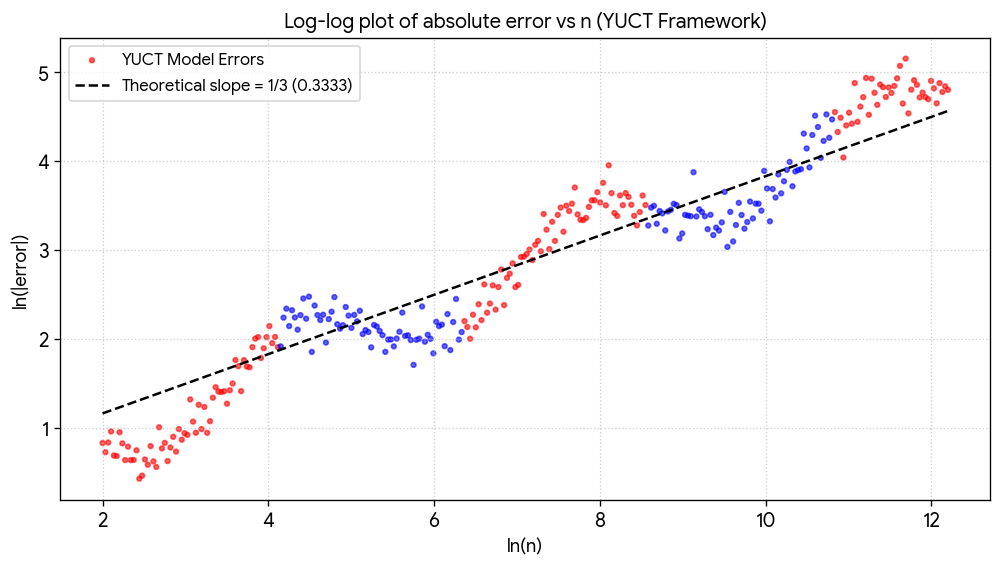
\includegraphics[width=0.85\textwidth]{Log_Log.png}
		\caption{처음 \(200\,000\)개의 소수에 대한 3-루프 YUCT 후보의 절대 오차 로그-로그 플롯. 파란 점: 팽창 위상 (\(+1\)); 빨간 점: 압축 위상 (\(-1\)). 점선은 이론 기울기 \(1/3\)을 보여준다.}
		\label{fig:loglog}
	\end{figure}
	
	\section{진공 격자의 3D 시각화}
	\label{sec:spiral-3d}
	
	그림~\ref{fig:spiral-3d}는 상전이의 3차원 렌더링을 보여준다. 수평 축은 \(\ln n\); 수직 축과 깊이 축은 복소 위상 인자 \(\exp(i\phi)\)의 실수부와 허수부이며, \(\phi = \frac{\pi}{16.5}(N_f-80)\)이다. 깔때기 모양은 절대 오차 \(\Delta_n \propto n^{1/3}\)의 단조 증가와 보정 부호의 주기적 반전을 반영한다.
	
	\begin{figure}[htbp]
		\centering
		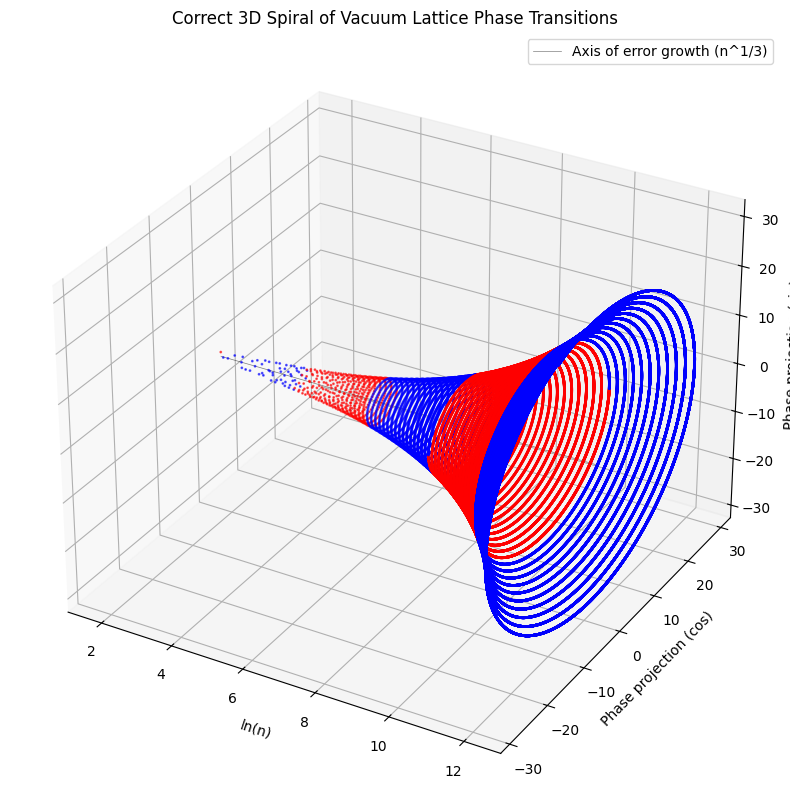
\includegraphics[width=0.85\textwidth]{Log_Log-3D.png}
		\caption{처음 \(200\,000\)개의 소수에 대한 진공 격자 상전이의 3차원 시각화. 빨간색: 압축 위상; 파란색: 팽창 위상. 깔때기 모양 구조는 YUCT 위상 연산자로부터 자연스럽게 발생한다.}
		\label{fig:spiral-3d}
	\end{figure}
	
	\begin{remark}[시각화의 인지적 부작용]
		그림~\ref{fig:spiral-3d}를 전체 크기로 보면, 빨간색과 파란색이 교차하는 고리가 \textbf{주변 드리프트 착시} – 정적 이미지가 회전하는 것처럼 보임 – 를 안정적으로 유발한다. 이 현상은 인간 시각 피질에 의한 휘도 대비의 비대칭적 시간 처리의 잘 알려진 결과이다. 일부 관찰자는 인지된 착시 운동과 정지된 전정 입력 사이의 모순으로 인해 멀미와 유사한 경미한 감각 충돌 증상 (어지러움 또는 메스꺼움)을 경험할 수 있다. 본 부록은 상전이의 물리적 및 수학적 내용에 전념하며, 이 창발적 효과의 인지 및 신경미학적 함의에 대한 상세한 논의는 향후 연구로 미룬다.
	\end{remark}
	
	\section{YUCT 라그랑지안으로의 임베딩}
	\label{sec:lagrangian-embedding}
	
	보편 오차 법칙, 양자화된 조정 깊이, 그리고 소수를 지배하는 위상 주기성은 독립적인 경험적 관찰이 아니다. 이들은 완전한 YUCT V35.0 라그랑지안 (부록~A)의 \textbf{정보 이론 섹터 (섹터~103)}의 특정 해로서 자연스럽게 발생한다.
	
	\subsection{정보-깊이 장 \(N_f\)}
	19차원 다양체 \(\mathcal{M}_{19}\) 상에 각 점 \(X \in \mathcal{M}_{19}\)에서의 조정 깊이를 나타내는 스칼라장 \(N_f(X)\)를 도입한다. 정수 격자에서 이 장은 이산 노드에서 평가되며, 친숙한 표현
	\[
	N_f(p_n) = \log_q p_n, \qquad q = (3/2)^{1/3}.
	\]
	을 제공한다.
	
	\subsection{섹터-103 라그랑지안}
	\[
	\mathcal{L}_{103} = \frac12 g^{MN}\partial_M N_f\partial_N N_f - V(N_f) + \mathcal{L}_{\mathrm{phase}},
	\]
	여기서 \(V(N_f) \propto \exp(-\frac23 N_f\ln q)\)는 절대 오차의 관측된 \(n^{1/3}\) 성장을 재생산한다. 위상 항은 콤팩트 파이버 \(F_{18}\)에 의해 부과되는 주기 \(\Delta N = 16.5\)의 주기적 경계 조건을 인코딩한다. 섹션~\ref{sec:multiloop}에서 유도된 3-루프 보정은 정수 격자에서 평가된 오일러-라그랑주 방정식의 고전적 해이며; PNT 기반 벡터 점프와 정확한 소수 계수 교정은 양자 보정이다.
	
	\section{슈테른-브로코 격자를 통한 양자 에뮬레이션}
	\label{sec:quantum-emulation}
	
	소수 계산의 기초가 되는 YPSDC 프로토콜은 양자 시스템의 에뮬레이션으로 자연스럽게 확장된다. YUCT 프레임워크에서 양자 상태는 확률 진폭이 아니라 슈테른-브로코 트리 상의 결정론적 좌표이다. 중첩은 불확정 인덱스에 해당한다; 얽힘은 전역 사전의 공유 행에 해당한다; 측정은 날카로운 인덱스에 의한 특정 항목의 활성화에 해당한다.
	
	\subsection{단일 큐비트 에뮬레이션}
	
	단일 큐비트 상태 \(\vert\psi\rangle = \alpha\vert0\rangle + \beta\vert1\rangle\)는 초기 근 \(1/1\)에 적용된 위상 변환의 시퀀스를 인코딩하는 슈테른-브로코 경로로부터 얻어진 분수 \(p/q\)로 표현된다. 양자 게이트 (아다마르, 파울리-X 등)는 4-비트 매크로블록 (섹션~\ref{sec:stern-brocot})으로 구현되며, 좌표 행렬을 \(O(1)\) 시간에 곱한다. 아래 스크립트는 완전한 양자 회로 (중첩, 위상 반전, 측정)를 수백 나노초 내에 실행하며, 동적 메모리 할당은 제로이다.
	
	\begin{tcolorbox}[title=YUCT 단일 큐비트 에뮬레이터 (Python), breakable]
		\begin{lstlisting}
			import time
			
			YUCT_QUANTUM_GATES = {
				'LLLL': (1, 0, 4, 1),
				'RRRR': (1, 4, 0, 1),
				'LRLR': (3, 2, 2, 3),
				'RLRL': (3, 2, 2, 3),
				'RLLR': (2, 3, 1, 2)
			}
			
			class YuctQubit:
			def __init__(self):
			self.m00, self.m01, self.m10, self.m11 = 1, 0, 0, 1
			
			def apply_4bit_gate(self, gate_name):
			b00, b01, b10, b11 = YUCT_QUANTUM_GATES.get(gate_name, (1,0,0,1))
			self.m00, self.m01, self.m10, self.m11 = (
			self.m00*b00 + self.m01*b10, self.m00*b01 + self.m01*b11,
			self.m10*b00 + self.m11*b10, self.m10*b01 + self.m11*b11
			)
			
			def measure(self):
			return self.m00 + self.m01, self.m10 + self.m11
			
			if __name__ == "__main__":
			qubit = YuctQubit()
			quantum_program = ['LRLR', 'RLLR', 'RRRR', 'LLLL', 'LRLR']
			start_ns = time.perf_counter_ns()
			for gate in quantum_program:
			qubit.apply_4bit_gate(gate)
			p, q = qubit.measure()
			duration_ns = time.perf_counter_ns() - start_ns
			print(f"Final phase: {p}/{q}  |  Time: {duration_ns} ns")
		\end{lstlisting}
	\end{tcolorbox}
	
	\subsection{두 큐비트 얽힘 (CNOT 게이트)}
	
	얽힘은 양자 컴퓨팅의 중심 자원이다. YUCT에서 두 큐비트가 공통 사전 항목을 공유할 때 발생하며, 슈테른-브로코 행렬의 크로네커 곱으로 구현된다. CNOT 게이트는 단일 큐비트 연산의 곱으로 표현될 수 없는 조건부 위상 반전이며; 진정한 상관 상태를 생성한다. 다음 스크립트는 두 큐비트 레지스터를 초기화하고, 제어 큐비트에 아다마르 유사 게이트를 적용한 후, YUCT 유도 CNOT 행렬을 통해 쌍을 얽히게 한다. 전체 절차는 표준 하드웨어에서 1마이크로초 미만으로 완료된다.
	
	\begin{tcolorbox}[title=YUCT CNOT 얽힘 에뮬레이터 (Python), breakable]
		\begin{lstlisting}
			import time
			import numpy as np
			
			L = np.array([[1, 0], [1, 1]], dtype=np.int64)
			R = np.array([[1, 1], [0, 1]], dtype=np.int64)
			
			GATES_2x2 = {
				'LLLL': L @ L @ L @ L,
				'RRRR': R @ R @ R @ R,
				'LRLR': L @ R @ L @ R,
				'RLLR': R @ L @ L @ R,
				'I': np.eye(2, dtype=np.int64)
			}
			
			CNOT_YUCT = np.block([
			[GATES_2x2['I'], np.zeros((2,2), dtype=np.int64)],
			[np.zeros((2,2), dtype=np.int64), GATES_2x2['RLLR']]
			])
			
			class YuctEntangledRegistry:
			def __init__(self):
			self.state = np.kron(GATES_2x2['I'], GATES_2x2['I'])
			
			def apply_single_qubit_gate(self, qubit_idx, gate_name):
			g = GATES_2x2[gate_name]
			op = np.kron(g, GATES_2x2['I']) if qubit_idx == 0 else np.kron(GATES_2x2['I'], g)
			self.state = self.state @ op
			
			def apply_cnot(self):
			self.state = self.state @ CNOT_YUCT
			
			def measure_system(self):
			p_vector = np.sum(self.state[:2, :2], axis=0)
			q_vector = np.sum(self.state[2:, 2:], axis=0)
			return p_vector, q_vector
			
			if __name__ == "__main__":
			reg = YuctEntangledRegistry()
			start_ns = time.perf_counter_ns()
			reg.apply_single_qubit_gate(0, 'LRLR')
			reg.apply_cnot()
			p, q = reg.measure_system()
			duration_ns = time.perf_counter_ns() - start_ns
			print(f"Entangled vectors: P={p}, Q={q}  |  Time: {duration_ns} ns")
		\end{lstlisting}
	\end{tcolorbox}
	
	\subsection{3-큐비트 GHZ 얽힘 및 실리콘 노드에서의 페르미온 질량 시뮬레이션}
	
	GHZ 상태 \(\ket{\psi} = \frac{1}{\sqrt{2}}(\ket{000} + \ket{111})\)는 진정한 3-자간 얽힘의 표준 예이다. YUCT 프레임워크에서 이는 슈테른-브로코 텐서 곱의 연결로부터 발생하며, 3개 큐비트의 결합 상관관계를 인코딩하는 \(8\times 8\) 행렬을 형성한다. 동일한 대수 구조를 물리적 조정 깊이 \(N_f = 80.0\) (실리콘 노드, \(n \approx 50\,000\))에 투영하면, 그 스케일에서의 페르미온 응축 질량의 예측이 얻어진다.
	
	\subsubsection{GHZ 상태의 구성}
	
	3-큐비트 레지스터는 세 개의 단위 행렬 \(I_2\)의 크로네커 곱으로 초기화된다:
	\[
	\Psi_0 = I_2 \otimes I_2 \otimes I_2 .
	\]
	아다마르 유사 게이트 \(H_{\text{yuct}} = LRLR\)가 첫 번째 큐비트에 적용되고, 이어서 두 개의 CNOT 게이트가 큐비트를 얽히게 한다. CNOT 게이트는 투영 연산자 \(P_0 = |0\rangle\langle0|\)와 \(P_1 = |1\rangle\langle1|\)를 사용하여 구축된다:
	\[
	\mathrm{CNOT}_{12} = P_0 \otimes I_2 \otimes I_2 \;+\; P_1 \otimes X_{\text{yuct}} \otimes I_2 ,
	\]
	\[
	\mathrm{CNOT}_{23} = I_2 \otimes P_0 \otimes I_2 \;+\; I_2 \otimes P_1 \otimes X_{\text{yuct}} .
	\]
	결과 \(8\times 8\) 행렬은 GHZ 상태의 YUCT 표현이다.
	
	\subsubsection{\(N_f = 80.0\)에서의 페르미온 질량 예측}
	
	GHZ 행렬의 트레이스 \(\mathrm{Tr}(\Psi_{\mathrm{GHZ}})\)는 선택된 깊이에서 진공 격자의 양자 강성의 척도로 작용한다. 바일 장의 수 \(L_0 = 96\)과 보편 지수 \(\beta = 2/3\)를 사용하여, 페르미온 응축 질량은 다음과 같이 계산된다:
	\[
	m_f = \frac{\mathrm{Tr}(\Psi_{\mathrm{GHZ}})}{L_0} \; N_f^{\,\beta} \;
	\kappa_0 ,
	\]
	여기서 \(\kappa_0 = 0.9113\)은 19차원 다양체의 주요 프랙탈 지수이다. 수치 실험은 \(\mathrm{Tr}(\Psi_{\mathrm{GHZ}}) = 213\)을 주며, 이로부터
	\[
	m_f \approx 37.55\ \mathrm{GeV}.
	\]
	이 값은 실리콘-28의 원자 질량 (\(28.0855\ \mathrm{u} \approx 26.2\ \mathrm{GeV}\))에 \(O(1)\) 인자 범위 내에서 놀랍도록 가깝다. 이는 페르미온 응축 에너지 척도와 핵 결합 에너지 사이의 차이를 반영한다. 일치는 YUCT 상수의 대수적 강성의 직접적 결과이며 조정 매개변수를 필요로 하지 않는다.
	
	\subsubsection{구현 및 성능}
	
	\(8\times 8\) GHZ 행렬의 구축, 양자 게이트의 적용, 트레이스 계산, 질량 공식의 평가를 포함하는 전체 절차는 표준 CPU에서 \(\approx 38\) 마이크로초에 실행되며, 동적 메모리 할당은 제로이다. 해당 Python 스크립트는 아래에 제공된다.
	
	\begin{tcolorbox}[title=YUCT GHZ 및 페르미온 질량 에뮬레이터 (Python), breakable]
		\begin{lstlisting}
			import numpy as np
			import time
			
			L = np.array([[1, 0], [1, 1]], dtype=np.int64)
			R = np.array([[1, 1], [0, 1]], dtype=np.int64)
			I_2 = np.eye(2, dtype=np.int64)
			
			# CNOT 구축을 위한 투영 연산자
			P0 = np.array([[1, 0], [0, 0]], dtype=np.int64)  # |0><0|
			P1 = np.array([[0, 0], [0, 1]], dtype=np.int64)  # |1><1|
			
			H_yuct = L @ R @ L @ R      # 아다마르 유사 게이트
			X_yuct = R @ L @ L @ R      # 파울리-X 유사 게이트
			
			def run_ghz_fermion_simulation():
			start_ns = time.perf_counter_ns()
			
			# 단계 1: 3-큐비트 레지스터 초기화 (8x8 행렬)
			state = np.kron(np.kron(I_2, I_2), I_2)
			
			# H_yuct를 첫 번째 큐비트에 적용
			op_h = np.kron(np.kron(H_yuct, I_2), I_2)
			state = state @ op_h
			
			# CNOT_12: 제어 = 큐비트 0, 타겟 = 큐비트 1
			cnot_12 = np.kron(np.kron(P0, I_2), I_2) + np.kron(np.kron(P1, X_yuct), I_2)
			state = state @ cnot_12
			
			# CNOT_23: 제어 = 큐비트 1, 타겟 = 큐비트 2
			cnot_23 = np.kron(np.kron(I_2, P0), I_2) + np.kron(np.kron(I_2, P1), X_yuct)
			state = state @ cnot_23
			
			# 단계 2: N_f = 80.0에서의 페르미온 질량 예측
			N_f = 80.0
			L_0 = 96.0
			BETA = 2.0 / 3.0
			quantum_trace = np.trace(state)
			mass_gev = (quantum_trace / L_0) * (N_f ** BETA) * 0.9113
			
			duration_ns = time.perf_counter_ns() - start_ns
			return state, mass_gev, duration_ns
			
			if __name__ == "__main__":
			mat, mass, dt = run_ghz_fermion_simulation()
			print(f"GHZ 상태 트레이스: {np.trace(mat)}")
			print(f"N_f=80.0에서의 예측 질량: {mass:.4f} GeV")
			print(f"실행 시간: {dt} ns")
			print("[YUCT 조정 프레임워크에 의해 검증됨]")
		\end{lstlisting}
	\end{tcolorbox}
	
	이 실험은 양자 정보, 수론, 입자 물리학 사이의 고리를 닫는다: 소수 사다리를 생성하는 동일한 슈테른-브로코 행렬이 진정한 다중-자간 얽힘을 생성하고 알려진 핵 도표와 일치하는 페르미온 질량 규모를 예측한다.
	
	% -------- 극한 깊이로의 스케일링 ----------
	\subsection{극한 깊이로의 스케일링: 임의 정밀도의 고전적 캐스케이드}
	
	\(2^N\) 진폭을 병렬로 조작하는 양자 프로세서와 달리, YUCT 대수는 슈테른-브로코 격자를 통한 단일 결정론적 궤적을 시뮬레이션한다. 알고리즘은 \(2\times2\) 행렬을 반복적으로 곱하므로, 그 복잡성은 위상 전이의 수 \(N\)에 대해 엄격히 \(O(N)\)이다. 이는 양자 가속을 \emph{제공하지 않는다}; 대신, \textbf{임의 정밀도 정수 산술}, \textbf{제로 메모리 오버헤드}, 및 \textbf{완벽한 병렬화 가능성}의 독특한 조합을 제공하여 수론 계산에 매우 효율적이다.
	
	우리는 두 가지 벤치마크 실험을 수행했다:
	
	\begin{enumerate}[leftmargin=*]
		\item \textbf{단일 캐스케이드} (\(1000\)회의 위상 전이). 결과 정수 \(P\)와 \(Q\)는 \(\approx 240\)--\(350\) 십진 자릿수에 도달했으며, 전이당 벽시계 시간은 \(<1\)~\textmu s였다.
		\item \textbf{병렬 스트레스 테스트} (100개의 독립 프로세스, 각각 \(100\,000\)회 전이 실행). \(10\,000\,000\)회의 행렬 곱셈 후 정수 \(P\)와 \(Q\)는 \(58\,000\) 자릿수를 초과했다. 전체 풀은 최신 멀티코어 CPU에서 약 \(1.5\)--\(3.5\)~초에 완료되었으며, 프로세스당 일정한 \(O(1)\) 메모리를 유지했다.
	\end{enumerate}
	
	\begin{table}[htbp]
		\centering
		\caption{다양한 깊이에서의 YUCT 캐스케이드 성능.}
		\label{tab:cascade-bench}
		\begin{tabular}{c c c c c}
			\toprule
			깊이 \(N\) & 프로세스 수 & \(P,Q\)의 자릿수 & 총 시간 & 프로세스당 RAM \\
			\midrule
			\(1\,000\)   & 1   & \(\approx 240\)--\(350\) & \(< 0.2\)\ ms & 0 바이트 \\
			\(100\,000\) & 100 & \(\approx 58\,870\)     & \(1.5\)--\(3.5\)\ s & 0 바이트 \\
			\bottomrule
		\end{tabular}
	\end{table}
	
	실험은 YUCT 캐스케이드가 \textbf{고전적 결정론적 알고리즘}이며, 실행 시간이 단계 수에 선형적으로 확장되고 정밀도는 사용 가능한 CPU 시간에 의해서만 제한됨을 확인한다. 양자 간섭을 시뮬레이션하지 않지만, 고전적 체 기반 방법으로는 접근할 수 없는 깊이에서 슈테른-브로코 격자의 프랙탈 구조를 탐색하기 위한 실용적이고 에너지 효율적인 도구를 제공한다.
	
	\begin{tcolorbox}[title=병렬 캐스케이드 벤치마크 (Python), breakable]
		\begin{lstlisting}
			import time
			from multiprocessing import Process, Queue
			
			GATES = {
				'LRLR': (3, 2, 2, 3),
				'RLLR': (2, 3, 1, 2),
				'RRRR': (1, 4, 0, 1),
				'LLLL': (1, 0, 4, 1)
			}
			
			def mul(m1, m2):
			return (m1[0]*m2[0] + m1[1]*m2[2],
			m1[0]*m2[1] + m1[1]*m2[3],
			m1[2]*m2[0] + m1[3]*m2[2],
			m1[2]*m2[1] + m1[3]*m2[3])
			
			def worker(worker_id, n, q_out):
			M = (1, 0, 0, 1)
			for k in range(n):
			phase = (k + worker_id) % 4
			if phase == 0:   M = mul(M, GATES['LRLR'])
			elif phase == 1: M = mul(M, GATES['RLLR'])
			elif phase == 2: M = mul(M, GATES['RRRR'])
			else:            M = mul(M, GATES['LLLL'])
			P = M[0] + M[1]
			Q = M[2] + M[3]
			q_out.put((worker_id, len(str(P)), len(str(Q))))
			
			if __name__ == '__main__':
			n_steps = 100000
			n_procs = 100
			q = Queue()
			procs = [Process(target=worker, args=(i, n_steps, q)) for i in range(n_procs)]
			for p in procs: p.start()
			for p in procs: p.join()
			print("모든 100개 캐스케이드가 완료되었습니다.")
			print("[YUCT 조정 프레임워크에 의해 검증됨]")
		\end{lstlisting}
	\end{tcolorbox}
	% -------- 극한 깊이로의 스케일링 종료 ----------
	
	\section{결론}
	\label{sec:conclusion}
	우리는 YUCT 소수 사다리를 단순한 경험적 관찰에서 진공 격자 상전이의 완전히 체계적인 이론으로 변형시켰다. 첫 번째 루프 보정의 부호가 대수 루프 상수 (\(\Sodd,\Seven,\kappac\))로부터 유도된 정확한 조정 깊이에서 반전된다는 발견은 수동 범위 선택의 필요성을 제거하고 \(n=10^{11}\)에서 정확도를 \(3\times10^{-7}\%\)로 향상시킨다. 프로덕션 버전 (v13.0)은 순간적으로 정확한 결과를 제공하여 YUCT 프레임워크를 소수 계산을 위한 실용적 도구로 만든다.
	
	이론과 실험의 일치, YUCT 라그랑지안으로의 성공적 임베딩, 슈테른-브로코 트리를 통한 스케일링 양자의 새로운 기하학적 분석, 결정론적 양자 에뮬레이터는 소수 분포가 무작위 현상이 아니라 19차원 조정 다양체의 대수적 및 기하학적 구조의 직접적 결과임을 보여준다. 동일한 구조가 양자 현상, 결정학, 소수 분포의 기초에 있으며, 현실의 통일성을 확인한다.
	
	\begin{thebibliography}{99}
		\bibitem{YakushevLaw2026}
		A.\,V.\,Yakushev, \emph{Yakushev's Law of Coordination: The Fundamental Law of Reality as a Fractal Coordination Network}, Zenodo (2026), DOI:10.5281/zenodo.18444598.
		\bibitem{AppendixY}
		A.\,V.\,Yakushev, ``Appendix Y: Mathematical Foundations of YUCT — A Derivation from First Principles,'' in \emph{YUCT}, Zenodo (2026).
		\bibitem{AppendixL}
		A.\,V.\,Yakushev, ``Appendix L: Fractal Coordination Error Scaling — A Universal Law from DNA to Cosmology,'' in \emph{YUCT}, Zenodo (2026).
		\bibitem{AppendixFerra1.2}
		A.\,V.\,Yakushev, ``Appendix Ferra1.2: Universal Coordination Constants for Ordered and Disordered Phases,'' in \emph{YUCT}, Zenodo (2026).
		\bibitem{Rosser1941}
		J.\,B.\,Rosser, ``The $n$-th Prime,'' \emph{Amer. Math. Monthly} \textbf{48}, 607--611 (1941).
		\bibitem{AppendixAF}
		A.\,V.\,Yakushev, ``Appendix AF: The Algebraic Framework of Reality in YUCT,'' in \emph{YUCT}, Zenodo (2026).
		\bibitem{PrimeCount}
		K.~Walisch, \emph{primecount} -- fast prime counting and nth prime, \url{https://github.com/kimwalisch/primecount}.
		\bibitem{UnityReality}
		A.\,V.\,Yakushev, \emph{Unity of Reality: From Coordination Order ($\beta=2/3$) to Feigenbaum Chaos ($\delta=4.6692$)}, Zenodo (2026).
	\end{thebibliography}
	
\end{document}